%!TEX root = ../vortrag.tex
\section{Das Umgebungsmodell}
\begin{frame}[t,fragile]{Rückblick: Substitutionsmodell}
	\begin{mybox}
		Um eine Prozedur auf konkrete Werte anzuwenden, ersetze im Rumpf der Prozedur jeden formalen Parameter mit dem entsprechenden Wert und werte den Rumpf aus.
	\end{mybox}
	
	\bet{Schwächen des Modells:}
	\begin{itemize}
		\item<2-> Unklarheiten bei mehrfacher Verwendung von gleichen Bezeichnern.
		\item<2-> Liefert ggfs. falsche Resultate bei Verwendung von Zuweisungen (imperative Programmierung).
		\item<2-> Berücksichtigt nicht, in welchem Kontext eine Prozedur definiert wurde.
	\end{itemize}
	\onslide<3->{\bet{Konsequenzen} für ein \textit{besseres} Modell:}
	\begin{itemize}
		\item<3-> Modell muss die \bet{Umgebung} berücksichtigen, in der eine Auswertung stattfindet.
		\item<3-> Notwendigkeit, für jede Prozedur die Umgebung zu speichern, in der sie definiert wurde.
	\end{itemize}	
	\onslide<4->{
	\begin{mybox}
		\bet{Definition:} Eine \bet{Umgebung} legt die Bedeutung von Bezeichnern fest.
		Sie umfasst, welcher Bezeichner an welchen eindeutig bestimmten Wert gebunden ist. \minor{(vgl. \cite[S. 187]{clausing})}
	\end{mybox}}
\end{frame}

\begin{frame}[t,fragile]{Umgebungsmodell -- Bindungsrahmen}
	\begin{itemize}
		\item Eine Umgebung kann aufgefasst werden als eine Folge von Bindungsrahmen.
		\item Ein Bindungsrahmen enthält Bindungen von Bezeichnern an eindeutig bestimmte Werte sowie einen Verweis auf die Umgebung, in der er entstanden ist.
		\item<2-> \bet{Beispiel:} Umgebung $U_1$ besteht aus dem einzigen Rahmen \texttt{I}. 		
			Umgebung $U_2$ besteht aus der Rahmenfolge \texttt{II} $\rightarrow$ \texttt{I}, $U_3$ wiederum aus \texttt{III} $\rightarrow$ \texttt{I}.
		
		\begin{center}
			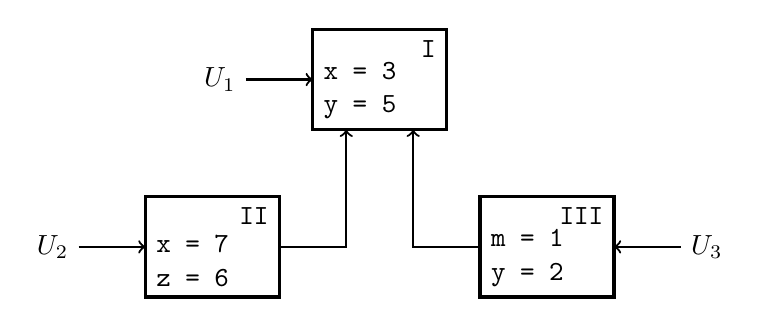
\begin{tikzpicture}[scale=0.85]
				\draw [very thick] (0,0) node[anchor=south west,align=left,font=\ttfamily]{x = 7 \\ z = 6}
					rectangle (2,1.5) node[anchor=north east]{\ttfamily II};
				\draw [very thick] (2.5,2.5) node[anchor=south west,align=left,font=\ttfamily]{x = 3 \\ y = 5}
				rectangle (4.5,4) node[anchor=north east]{\ttfamily I};
				\draw [thick,->] (1.5,3.25) node[left]{$U_1$} -- (2.5,3.25);
				\draw [very thick] (5,0) node[anchor=south west,align=left,font=\ttfamily]{m = 1 \\ y = 2}
				rectangle (7,1.5) node[anchor=north east]{\ttfamily III};
				\draw [thick,->] (2,0.75) -- (3,0.75) -- (3,2.5);
				\draw [thick,->] (5,0.75) -- (4,0.75) -- (4,2.5);
				\draw [thick,->] (-1,0.75) node[left]{$U_2$} -- (0,0.75);
				\draw [thick,->] (8,0.75) node[right]{$U_3$} -- (7,0.75);	
			\end{tikzpicture}
		\end{center}
	\end{itemize}
\end{frame}

\begin{frame}[t,fragile]{Werte von Variablen}
	\begin{mybox}
		Der Wert einer Variablen bezüglich einer Umgebung ist bestimmt durch den ersten Rahmen, in dem die Variable an einen Wert gebunden ist.
	\end{mybox}
	
	\vspace*{0.5cm}

	\begin{minipage}{0.5\textwidth}
	\begin{itemize}
		\item<2-> Wert von \texttt{x} in der Umgebung $U_1$: \quad \texttt{3}
		\item<3-> Wert von \texttt{x} in der Umgebung $U_2$: \quad \texttt{7}
		\item<3-> Die Bindung von \texttt{x} im Rahmen \texttt{I} wird durch die Bindung in Rahmen \texttt{II} \bet{maskiert}.
		\item<4-> Wert von \texttt{x} in der Umgebung $U_3$: \quad \texttt{3}
		\item<5-> Aus Sicht der Umgebung $U_1$ bzw. $U_2$ \\ ist \texttt{m} nicht gebunden.
	\end{itemize}
	\end{minipage}~\begin{minipage}{0.5\textwidth}
		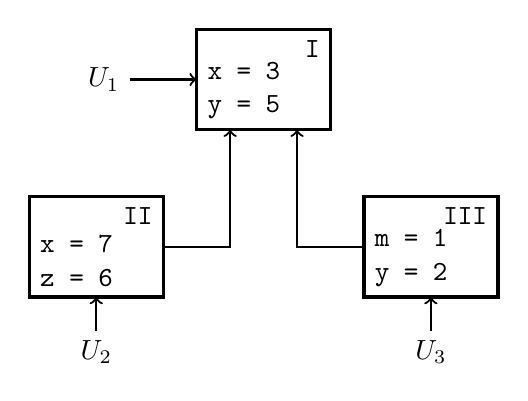
\begin{tikzpicture}[scale=0.85]
			\draw [very thick] (0,0) node[anchor=south west,align=left,font=\ttfamily]{x = 7 \\ z = 6}
				rectangle (2,1.5) node[anchor=north east]{\ttfamily II};
			\draw [very thick] (2.5,2.5) node[anchor=south west,align=left,font=\ttfamily]{x = 3 \\ y = 5}
			rectangle (4.5,4) node[anchor=north east]{\ttfamily I};
			\draw [thick,->] (1.5,3.25) node[left]{$U_1$} -- (2.5,3.25);
			\draw [very thick] (5,0) node[anchor=south west,align=left,font=\ttfamily]{m = 1 \\ y = 2}
			rectangle (7,1.5) node[anchor=north east]{\ttfamily III};		
			\draw [thick,->] (2,0.75) -- (3,0.75) -- (3,2.5);
			\draw [thick,->] (5,0.75) -- (4,0.75) -- (4,2.5);
			\draw [thick,->] (1,-0.5) node[below]{$U_2$} -- (1,0);
			\draw [thick,->] (6,-0.5) node[below]{$U_3$} -- (6,0);	
		\end{tikzpicture}
	\end{minipage}
\end{frame}

\begin{frame}[t,fragile]{Globale Umgebung}
	\begin{itemize}
		\item Die globale Umgebung $\mathcal{G}$ existiert beim Start des Interpreters und enthält sämtliche vordefinierte Bezeichner in einem einzigen Rahmen.
		\item Alle weiteren Umgebungen enden in diesem Rahmen.
		
		\vspace*{0.25cm}
		
		\begin{center}
			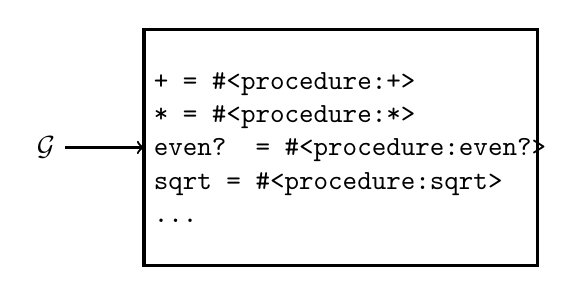
\begin{tikzpicture}
				\draw [very thick] (0,-0.5) rectangle (5,2.5);
				\draw [thick,->] (-1,1) node[left]{$\mathcal{G}$} -- (0,1);
				\draw (0,1) node[right,align=left,font=\ttfamily]{+ = \#<procedure:+> \\
					* = \#<procedure:*> \\
					even? = \#<procedure:even?> \\
					sqrt = \#<procedure:sqrt> \\ \dots};
			\end{tikzpicture}
		\end{center}
		\item \mintinline{scheme}{define} fügt Bindungen zum Rahmen der globalen Umgebung hinzu.
			Diese Bindungen sind daher für alle Umgebungen sichtbar.
	\end{itemize}
\end{frame}

\begin{frame}[t,fragile]{}
	\begin{itemize}
		\item \mintinline{scheme}{define} fügt Bindungen zum Rahmen der globalen Umgebung hinzu.
			Diese Bindungen sind daher für alle Umgebungen sichtbar.
	\end{itemize}
	\begin{minted}{scheme}
		(define antwort 42)
		(define pi 3.14)
	\end{minted}
	
	\begin{center}
		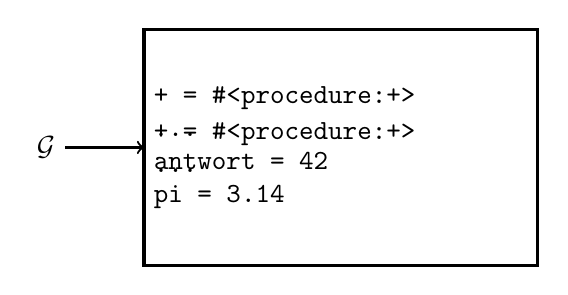
\begin{tikzpicture}
			\draw [very thick] (0,-0.5) rectangle (5,2.5);
			\draw [thick,->] (-1,1) node[left]{$\mathcal{G}$} -- (0,1);
			\draw<1|handout:0> (0,1) node[right,align=left,font=\ttfamily]{+ = \#<procedure:+> \\ \dots};
			\draw<2-> (0,1) node[right,align=left,font=\ttfamily]{+ = \#<procedure:+> \\ \dots \\ antwort = 42 \\ pi = 3.14};
		\end{tikzpicture}
	\end{center}
\end{frame}

\begin{frame}[t,fragile]{Definition von Prozeduren -- \textit{revisited}}
	\begin{itemize}
		\minoritem \minor{Notwendigkeit, für jede Prozedur die Umgebung zu speichern, in der sie definiert wurde}
		\item<2-> Ab jetzt: Betrachte eine Prozedur als Paar bestehend aus ihrer Definition $\lambda$ (Parameter und Rumpf) und einem Verweis auf die Umgebung $\mathcal{U}$, in der sie mittels \mintinline{scheme}{lambda}-Ausdruck erzeugt wurde.
		\begin{minted}{scheme}
			(define (square x) (* x x))		;; (define square (lambda (x) (* x x)))
		\end{minted}
		\item<3-> \mintinline{scheme}{define} hinterlegt Verweis auf dieses Paar im Bindungsrahmen.
	\end{itemize}
	\begin{center}
		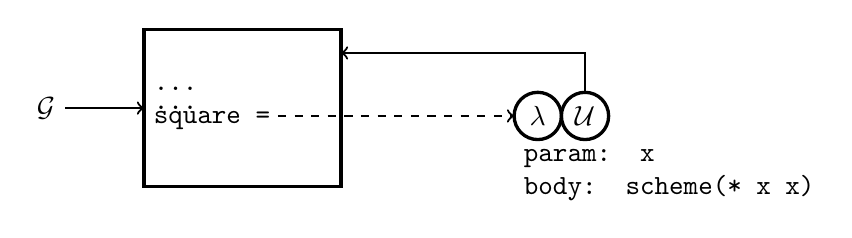
\begin{tikzpicture}
			\draw [very thick] (0,0) rectangle (2.5,2);
			\draw [thick,->] (-1,1) node[left]{$\mathcal{G}$} -- (0,1);
			\draw<1-2|handout:0> (0,1) node[right,align=left,font=\ttfamily]{\dots};
			\draw<3-> (0,1) node[right,align=left,font=\ttfamily]{\dots \\ square = };
			
			\onslide<2->{
				\draw[very thick] (5,0.9) node{$\lambda$} circle (0.3);
				\draw[very thick] (5.6,0.9) node{$\mathcal{U}$} circle (0.3);
				\draw (4.7,0.6) node[anchor=north west,align=left,font=\ttfamily]{param: x \\ body: \mintinline{scheme}{(* x x)}};
				\draw[thick,->] (5.6,1.2) -- (5.6,1.7) -- (2.5,1.7);}
			
			\draw<3-> [thick,dashed,->] (1.7,0.9) -- (4.7,0.9);
		\end{tikzpicture}
	\end{center}
\end{frame}

\begin{frame}[t,fragile]{Auswertung von Prozeduraufrufen}
	\begin{mybox}
		Um eine Prozedur auszuwerten, die in der Umgebung $\mathcal{U}$ erzeugt wurde, verfahre wie folgt: \ccite{sicp}{S. 239f}
		\begin{enumerate}
			\item Erzeuge eine neue Umgebung mit neuem Bindungsrahmen, der an die Umgebung $\mathcal{U}$ angehängt wird.
			\item Binde die formalen Parameter im erstellten Rahmen an die Aufrufparameter.
			\item Werte den Rumpf in der erzeugten Umgebung aus.
		\end{enumerate}
	\end{mybox}
	\begin{center}
		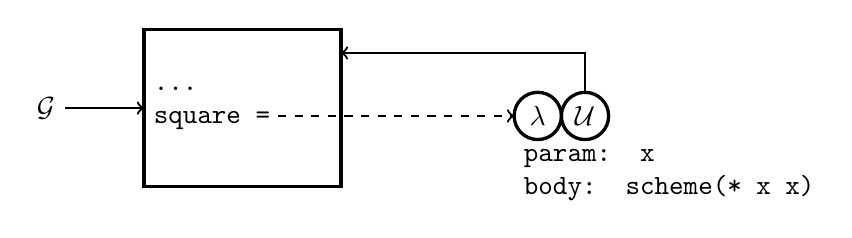
\begin{tikzpicture}
			\draw [very thick] (0,0) rectangle (2.5,2);
			\draw [thick,->] (-1,1) node[left]{$\mathcal{G}$} -- (0,1);
			\draw (0,1) node[right,align=left,font=\ttfamily]{\dots \\ square = };
			
			\draw[very thick] (5,0.9) node{$\lambda$} circle (0.3);
			\draw[very thick] (5.6,0.9) node{$\mathcal{U}$} circle (0.3);
			\draw (4.7,0.6) node[anchor=north west,align=left,font=\ttfamily]{param: x \\ body: \mintinline{scheme}{(* x x)}};
			\draw[thick,->] (5.6,1.2) -- (5.6,1.7) -- (2.5,1.7);
			
			\draw [thick,dashed,->] (1.7,0.9) -- (4.7,0.9);
		\end{tikzpicture}
	\end{center}	
	
\end{frame}

\begin{frame}[t,fragile]{}
	\bet{Beispiel 1:} Auswertung von \mintinline{scheme}{(square 7)}:
	\begin{mybox}
		\begin{itemize}
			\only<1-2|handout:1-2>{\item Erzeuge eine neue Umgebung mit neuem Bindungsrahmen, der an die Umgebung $\mathcal{U}$ angehängt wird.}
			\only<3|handout:3>{\item Binde die formalen Parameter im erstellten Rahmen an die Aufrufparameter.}
			\only<4-|handout:4>{\item Werte den Rumpf in der erzeugten Umgebung aus.}
		\end{itemize}
	\end{mybox}
	
	\only<3->{\vspace*{1.1em}}
	
	\begin{center}
		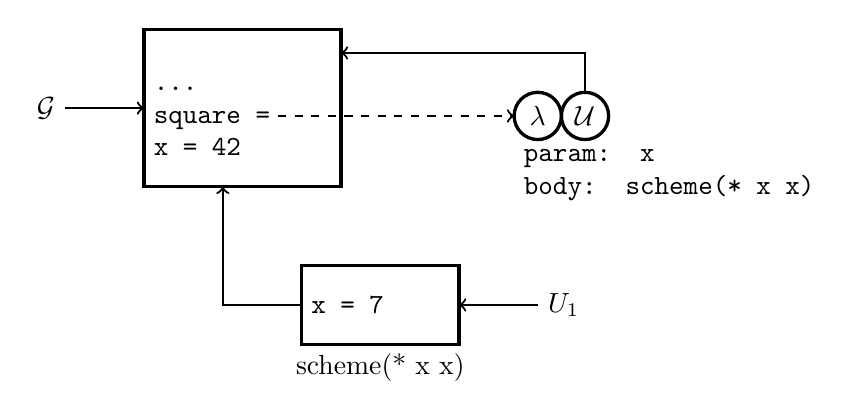
\begin{tikzpicture}
			\draw [very thick] (0,0) rectangle (2.5,2);
			\draw [thick,->] (-1,1) node[left]{$\mathcal{G}$} -- (0,1);
			\draw (0,1) node[right,align=left,font=\ttfamily]{\dots \\ square = };
			
			\draw[very thick] (5,0.9) node{$\lambda$} circle (0.3);
			\draw[very thick] (5.6,0.9) node{$\mathcal{U}$} circle (0.3);
			\draw (4.7,0.6) node[anchor=north west,align=left,font=\ttfamily]{param: x \\ body: \mintinline{scheme}{(* x x)}};
			\draw[thick,->] (5.6,1.2) -- (5.6,1.7) -- (2.5,1.7);
			\draw [thick,dashed,->] (1.7,0.9) -- (4.7,0.9);
			
			\onslide<2-|handout:2->{
				\draw [very thick] (2,-2) rectangle (4,-1);
				\draw [thick,->] (2,-1.5) -- (1,-1.5) -- (1,0);
				\draw [thick,->] (5,-1.5) node[right]{$U_1$} -- (4,-1.5);
				\draw (3,-2) node[below]{\mintinline{scheme}{(* x x)}};
			}
			
			\draw<3-|handout:3-> (2,-1.5) node[right,font=\ttfamily]{x = 7};
			\draw<5-|handout:0> (0,0.5) node[right,align=left,font=\ttfamily]{x = 42};
		\end{tikzpicture}
	\end{center}
	\begin{itemize}
		\item<4-|handout:4-> Wert von \texttt{x} in $U_1$ ist 7, daher wertet der Ausdruck zu 49 aus.
	\end{itemize}
\end{frame}

\begin{frame}[t,fragile,plain]{}
	\bet{Beispiel 2:} Auswertung von \mintinline{scheme}{((add-fun square cube) 5)} \minor{(vgl. Folie~\ref{folie:add-fun-eval})}:
	\begin{center}
		\begin{tikzpicture}
			%\draw [gray] (0,2) grid (12,-6);
			
			% global env
			\draw [very thick] (0,0) rectangle (3,2);
			\draw [thick,->] (-0.5,1) node[left]{$\mathcal{G}$} -- (0,1);
			\draw (0,1) node[right,align=left,font=\ttfamily]{\dots \\ add-fun = \\ cube = \\ square =  };
			
			% lambda square
			\draw[very thick] (0.3,-2) node{$\lambda$} circle (0.3);
			\draw[very thick] (0.9,-2) node{$\mathcal{U}$} circle (0.3);
			\draw (0,-2.3) node[anchor=north west,align=left,font=\ttfamily]{param: x \\ body: \mintinline{scheme}{(* x x)}};
			\draw [thick,->] (0.9,-1.7) -- (0.9,0);
			\draw [thick,dashed,->] (1.8,0.5) -- (2.5,0.5) -- (2.5,-0.5) -- (0.3,-0.5) -- (0.3,-1.7);
			
			% lambda cube
			\draw[very thick] (3.5,-2) node{$\lambda$} circle (0.3);
			\draw[very thick] (4.1,-2) node{$\mathcal{U}$} circle (0.3);
			\draw (3,-2.3) node[anchor=north west,align=left,font=\ttfamily]{param: x \\ body: \mintinline{scheme}{(* x x x)}};
			\draw [thick] (4.1,-1.7) -- (4.1,1.9);
			\draw [thick,dashed,->] (1.3,0.9) -- (3.5,0.9) -- (3.5,-1.7);
			
			% lambda add-fun
			\draw[very thick] (8,1.3) node{$\lambda$} circle (0.3);
			\draw[very thick] (8.6,1.3) node{$\mathcal{U}$} circle (0.3);
			\draw (7,1) node[anchor=north west,align=left,font=\ttfamily]{param: f, g \\ body: \mintinline{scheme}{(lambda (x) (+ (f x) (g x)))}};
			\draw[thick,->] (8.6,1.6) -- (8.6,1.9) -- (3,1.9);
			\draw [thick,dashed,->] (1.9,1.3) -- (7.7,1.3);
			
			% env add-fun
			\onslide<2-|handout:2->{
				\draw [very thick] (9,-0.5) rectangle (11,-1.5);
				\draw [thick,->] (11.5,-1.0) node[right]{$U_1$} -- (11,-1);
				\draw (9,-1) node[right,align=left,font=\ttfamily]{f = square \\ g = cube};
				\draw (10.5,-1.5) node[below]{\mintinline{scheme}{(lambda (x) (+ (f x) (g x)))}};
				\draw [thick] (9,-0.75) -- (6.5,-0.75) -- (6.5,1.9);
			}
			
			% result add-fun
			\onslide<3|handout:3>{
				\draw[very thick] (7,-2.5) node{$\lambda$} circle (0.3);
				\draw[very thick] (7.6,-2.5) node{$\mathcal{U}$} circle (0.3);
				\draw (6.7,-2.8) node[anchor=north west,align=left,font=\ttfamily]{param: x \\ body: \mintinline{scheme}{(+ (square x) (cube x))}};
				\draw[thick,->] (7.6,-2.2) -- (7.6,-1.2) -- (9,-1.2);
			}
			
			% env result add-fun
			\onslide<4-|handout:4->{
				\draw [very thick] (9,-3.5) rectangle (11,-4.5);
				\draw [thick,->] (11.5,-4.0) node[right]{$U_2$} -- (11,-4);
				\draw (9,-4) node[right,align=left,font=\ttfamily]{x = 5};
				\draw (10,-4.5) node[below]{\mintinline{scheme}{(+ (square x) (cube x))}};
				\draw [thick,->] (9,-4) -- (7.7,-4) -- (7.7,-1.2) -- (9,-1.2);
			}
			
			% env square
			\onslide<5-|handout:5->{
				\draw [very thick] (0,-4) rectangle (2,-5);
				\draw [thick,->] (-0.5,-4.5) node[left]{$U_3$} -- (0,-4.5);
				\draw (0,-4.5) node[right,align=left,font=\ttfamily]{x = 5};
				\draw (1,-5) node[below]{\mintinline{scheme}{(* x x)}};
				\draw [thick] (1,-4) -- (1,-3.5) -- (2.8,-3.5) -- (2.8,-1) -- (0.9,-1);
			}
			
			% env cube
			\onslide<6-|handout:6->{
				\draw [very thick] (5,-4) rectangle (7,-5);
				\draw [thick,->] (4.5,-4.5) node[left]{$U_4$} -- (5,-4.5);
				\draw (5,-4.5) node[right,align=left,font=\ttfamily]{x = 5};
				\draw (6,-5) node[below]{\mintinline{scheme}{(* x x x)}};
				\draw [thick] (6,-4) -- (6,-1) -- (4.1,-1);
			}
			
			\draw<1|handout:1> (0,-6) node[right]{{\footnotesize \textcolor{maincolor}{$\blacktriangleright$}} \quad
				Werte zunächst \mintinline{scheme}{(add-fun square cube)} aus.};
			\draw<2|handout:2> (0,-6) node[right]{{\footnotesize \textcolor{maincolor}{$\blacktriangleright$}} \quad
				Auswertung von \mintinline{scheme}{(add-fun square cube)} erzeugt neue Umgebung.};
			\draw<3|handout:3> (0,-6) node[right]{{\footnotesize \textcolor{maincolor}{$\blacktriangleright$}} \quad
				Auswertungsergebnis ist nicht-gebundene Prozedur.};
			\draw<4|handout:4> (0,-6) node[right]{{\footnotesize \textcolor{maincolor}{$\blacktriangleright$}} \quad
				Auswertung der nicht gebundenen Prozedur erzeugt neue Umgebung.};
			\draw<5|handout:5> (0,-6) node[right]{{\footnotesize \textcolor{maincolor}{$\blacktriangleright$}} \quad
				Auswertung von \mintinline{scheme}{(square 5)} erzeugt neue Umgebung.};
			\draw<6|handout:6> (0,-6) node[right]{{\footnotesize \textcolor{maincolor}{$\blacktriangleright$}} \quad
				Auswertung von \mintinline{scheme}{(cube 5)} erzeugt neue Umgebung.};
		\end{tikzpicture}
	\end{center}
\end{frame}

\begin{frame}[t,fragile]{Letztes Beispiel}
	\begin{minted}{scheme}
		(define (new-accu init)
			(lambda (x)
				(set! init (+ init x))
				init)))
				
		> (define accu1 (new-accu 100))
		> (accu1 10)
		110
		> (accu1 50)
		160	
	\end{minted}
	
	\begin{center}
		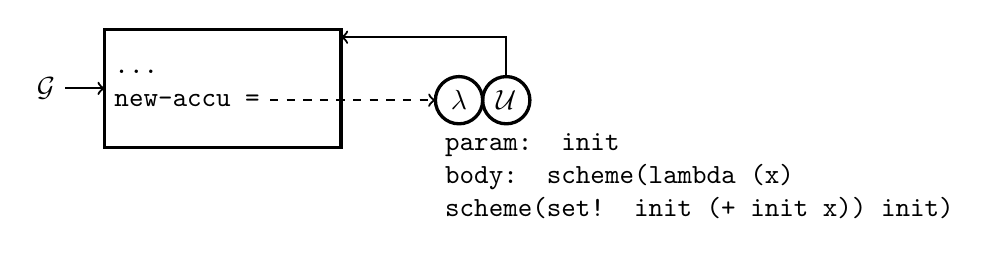
\begin{tikzpicture}
			%\draw [gray] (0,2) grid (10,-2);
			
			% global env
			\draw [very thick] (0,0) rectangle (3,1.5);
			\draw [thick,->] (-0.5,0.75) node[left]{$\mathcal{G}$} -- (0,0.75);
			\draw (0,0.75) node[right,align=left,font=\ttfamily]{\dots \\ new-accu = };
			
			% lambda new-accu
			\draw[very thick] (4.5,0.6) node{$\lambda$} circle (0.3);
			\draw[very thick] (5.1,0.6) node{$\mathcal{U}$} circle (0.3);
			\draw (4.2,0.3) node[anchor=north west,align=left,font=\ttfamily]{param: init \\ body: \mintinline{scheme}{(lambda (x)} \\ \mintinline{scheme}{(set! init (+ init x)) init)}};
			\draw [thick,->] (5.1,0.9) -- (5.1,1.4) -- (3,1.4);
			\draw [thick,dashed,->] (2.1,0.6) -- (4.2,0.6);
		\end{tikzpicture}
	\end{center}
\end{frame}

\begin{frame}[t,fragile,plain]{}
	\bet{Beispiel 3:} Auswertung von \mintinline{scheme}{(define accu1 (new-accu 100)) (accu1 10) (accu1 50)}:
	\begin{center}
		\begin{tikzpicture}
			%\draw [gray] (0,2) grid (12,-6);
			
			% global env
			\draw [very thick] (0,0) rectangle (3,1.5);
			\draw [thick,->] (-0.5,0.75) node[left]{$\mathcal{G}$} -- (0,0.75);
			\draw<1-3|handout:1-3> (0,0.75) node[right,align=left,font=\ttfamily]{\dots \\ new-accu = };
			\draw<4-|handout:4-> (0,0.75) node[right,align=left,font=\ttfamily]{\dots \\ new-accu = \\ accu1 = };
			
			% lambda new-accu
			\draw[very thick] (4.5,0.6) node{$\lambda$} circle (0.3);
			\draw[very thick] (5.1,0.6) node{$\mathcal{U}$} circle (0.3);
			\draw (3.2,0.3) node[anchor=north west,align=left,font=\ttfamily\footnotesize]{param: init \\ body: \mintinline[fontsize=\footnotesize]{scheme}{(lambda (x)} \\ \mintinline[fontsize=\footnotesize]{scheme}{(set! init (+ init x)) init)}};
			\draw [thick,->] (5.1,0.9) -- (5.1,1.4) -- (3,1.4);
			\draw<1-3|handout:1-3> [thick,dashed,->] (2.1,0.6) -- (4.2,0.6);
			\draw<4-|handout:4-> [thick,dashed,->] (2.1,0.85) -- (3.5,0.85) -- (3.5,0.6) -- (4.2,0.6);
			
			% env new-accu
			\onslide<2-|handout:2->{
				\draw [very thick] (9.5,0.5) rectangle (11.5,1.5);
				\draw [thick,->] (12,1) node[right]{$U_1$} -- (11.5,1);
				\draw<2-5|handout:2-5> (9.5,1) node[right,align=left,font=\ttfamily\footnotesize]{init = 100};
				\draw<6-8|handout:6-8> (9.5,1) node[right,align=left,font=\ttfamily\footnotesize]{init = \alert<6|handout:handout:6>{110}};
				\draw<9-|handout:9-> (9.5,1) node[right,align=left,font=\ttfamily\footnotesize]{init = \alert<9|handout:9>{160}};
				\draw (10.5,0.5) node[below]{\mintinline[fontsize=\footnotesize]{scheme}{(lambda (x) ...)}};
				\draw [thick] (9.5,1.4) -- (5.1,1.4);
			}
			
			% lambda accu1
			\onslide<3-|handout:3->{
				\draw[very thick] (9,-1.5) node{$\lambda$} circle (0.3);
				\draw[very thick] (9.6,-1.5) node{$\mathcal{U}$} circle (0.3);
				\draw (8.2,-1.8) node[anchor=north west,align=left,font=\ttfamily\footnotesize]{param: x \\ body: \mintinline[fontsize=\footnotesize]{scheme}{(set! init (+ init x)) init}};
				\draw [thick,->] (9.6,-1.2) -- (9.6,-0.5) -- (8.6,-0.5) -- (8.6,0.8) -- (9.5,0.8);
			}
			\onslide<4-|handout:4->{
				\draw [thick,dashed,->] (1.5,0.4) -- (2.8,0.4) -- (2.8,-1.5) -- (8.7,-1.5);
			}
			
			% env (accu1 10)
			\onslide<5-6|handout:5-6>{
				\draw [very thick] (9.5,-4.5) rectangle (11.5,-3.5);
				\draw [thick,->] (12,-4) node[right]{$U_2$} -- (11.5,-4);
				\draw (9.5,-4) node[right,align=left,font=\ttfamily\footnotesize]{x = 10};
				\draw (10.5,-4.5) node[below]{\mintinline[fontsize=\footnotesize]{scheme}{(set! init ...)}};
				\draw [thick] (9.5,-4) -- (7.7,-4) -- (7.7,0.8) -- (8.6,0.8);
			}
			
			% env (accu1 10)
			\onslide<8-9|handout:8-9>{
				\draw [very thick] (9.5,-4.5) rectangle (11.5,-3.5);
				\draw [thick,->] (12,-4) node[right]{$U_3$} -- (11.5,-4);
				\draw (9.5,-4) node[right,align=left,font=\ttfamily\footnotesize]{x = 50};
				\draw (10.5,-4.5) node[below]{\mintinline[fontsize=\footnotesize]{scheme}{(set! init ...)}};
				\draw [thick] (9.5,-4) -- (7.7,-4) -- (7.7,0.8) -- (8.6,0.8);
			}
			
			\draw<1|handout:1> (0,-6) node[right]{{\footnotesize \textcolor{maincolor}{$\blacktriangleright$}} \quad
				Werte zunächst \mintinline{scheme}{(new-accu 100)} aus.};
			\draw<2|handout:2> (0,-6) node[right]{{\footnotesize \textcolor{maincolor}{$\blacktriangleright$}} \quad
				Auswertung von \mintinline{scheme}{(new-accu 100)} erzeugt neue Umgebung.};
			\draw<3|handout:3> (0,-6) node[right]{{\footnotesize \textcolor{maincolor}{$\blacktriangleright$}} \quad
				Auswertungsergebnis ist Prozedur\dots};
			\draw<4|handout:4> (0,-6) node[right]{{\footnotesize \textcolor{maincolor}{$\blacktriangleright$}} \quad
				\dots die an den Bezeichner \texttt{accu1} gebunden wird.};
			\draw<5|handout:5> (0,-6) node[right]{{\footnotesize \textcolor{maincolor}{$\blacktriangleright$}} \quad
				Auswertung von \mintinline{scheme}{(accu1 10)} erzeugt neue Umgebung.};
			\draw<6|handout:6> (0,-6) node[right]{{\footnotesize \textcolor{maincolor}{$\blacktriangleright$}} \quad
				Bezeichner \texttt{init} wird in $U_1$ gefunden und manipuliert.};
			\draw<7|handout:7> (0,-6) node[right]{{\footnotesize \textcolor{maincolor}{$\blacktriangleright$}} \quad
				Auswertung von \mintinline{scheme}{(accu1 10)} beendet.};
			\draw<8|handout:8> (0,-6) node[right]{{\footnotesize \textcolor{maincolor}{$\blacktriangleright$}} \quad
				Auswertung von \mintinline{scheme}{(accu1 50)} erzeugt neue Umgebung.};
			\draw<9|handout:9> (0,-6) node[right]{{\footnotesize \textcolor{maincolor}{$\blacktriangleright$}} \quad
				Bezeichner \texttt{init} wird in $U_1$ gefunden und manipuliert.};
			\draw<10|handout:10> (0,-6) node[right]{{\footnotesize \textcolor{maincolor}{$\blacktriangleright$}} \quad
				Auswertung von \mintinline{scheme}{(accu1 50)} beendet.};
		\end{tikzpicture}
	\end{center}
\end{frame}

\begin{frame}[t,fragile,plain]{}
	Erzeugung eines neuen Akkumulators mit \mintinline{scheme}{(define accu2 (new-accu 500))}:
	\begin{center}
		\begin{tikzpicture}
			%\draw [gray] (0,2) grid (12,-6);
			
			% global env
			\draw<1-2|handout:1-2> [very thick] (0,0) rectangle (3,1.5);
			\draw<3-|handout:3-> [very thick] (0,-0.5) rectangle (3,1.5);
			\draw [thick,->] (-0.5,0.75) node[left]{$\mathcal{G}$} -- (0,0.75);
			\draw<1-2|handout:1-2> (0,0.75) node[right,align=left,font=\ttfamily]{\dots \\ new-accu = \\ accu1 = };
			\draw<3-|handout:3-> (0,0.55) node[right,align=left,font=\ttfamily]{\dots \\ new-accu = \\ accu1 = \\ accu2 = };
			
			% lambda new-accu
			\draw[very thick] (4.5,0.6) node{$\lambda$} circle (0.3);
			\draw[very thick] (5.1,0.6) node{$\mathcal{U}$} circle (0.3);
			\draw (3.2,0.3) node[anchor=north west,align=left,font=\ttfamily\footnotesize]{param: init \\ body: \mintinline[fontsize=\footnotesize]{scheme}{(lambda (x)} \\ \mintinline[fontsize=\footnotesize]{scheme}{(set! init (+ init x)) init)}};
			\draw [thick,->] (5.1,0.9) -- (5.1,1.4) -- (3,1.4);
			\draw [thick,dashed,->] (2.1,0.9) -- (3.5,0.9) -- (3.5,0.6) -- (4.2,0.6);
			
			% env new-accu
			\draw [very thick] (9.5,0.5) rectangle (11.5,1.5);
			\draw [thick,->] (12,1) node[right]{$U_1$} -- (11.5,1);
			\draw (9.5,1) node[right,align=left,font=\ttfamily\footnotesize]{init = 160};
			\draw (10.5,0.5) node[below]{\mintinline[fontsize=\footnotesize]{scheme}{(lambda (x) ...)}};
			\draw [thick] (9.5,1.4) -- (5.1,1.4);
			
			
			% lambda accu1
			\draw[very thick] (9,-1.5) node{$\lambda$} circle (0.3);
			\draw[very thick] (9.6,-1.5) node{$\mathcal{U}$} circle (0.3);
			\draw (8.2,-1.8) node[anchor=north west,align=left,font=\ttfamily\footnotesize]{param: x \\ body: \mintinline[fontsize=\footnotesize]{scheme}{(set! init (+ init x)) init}};
			\draw [thick,->] (9.6,-1.2) -- (9.6,-0.5) -- (8.6,-0.5) -- (8.6,0.8) -- (9.5,0.8);
			\draw [thick,dashed,->] (1.5,0.4) -- (2.8,0.4) -- (2.8,-1.5) -- (8.7,-1.5);
			
			% env new-accu
			\onslide<2-|handout:2->{
				\draw [very thick] (0,-3) rectangle (2,-4);
				\draw [thick,->] (-0.5,-3.5) node[left]{$U_4$} -- (0,-3.5);
				\draw (0,-3.5) node[right,align=left,font=\ttfamily\footnotesize]{init = 500};
				\draw (1,-4) node[below]{\mintinline[fontsize=\footnotesize]{scheme}{(lambda (x) ...)}};
				\draw<2|handout:2> [thick,->] (0.5,-3) -- (0.5,0);
				\draw<3-|handout:3-> [thick,->] (0.5,-3) -- (0.5,-0.5);
			}
			
			% lambda accu2
			\onslide<3-|handout:3->{
				\draw[very thick] (3.5,-3.5) node{$\lambda$} circle (0.3);
				\draw[very thick] (4.1,-3.5) node{$\mathcal{U}$} circle (0.3);
				\draw (3.2,-3.8) node[anchor=north west,align=left,font=\ttfamily\footnotesize]{param: x \\ body: \mintinline[fontsize=\footnotesize]{scheme}{(set! init (+ init x)) init}};
				\draw [thick,->] (4.1,-3.2) -- (4.1,-2.5) -- (1.5,-2.5) -- (1.5,-3);
				\draw [thick,dashed,->] (1.5,0) -- (2.2,0) -- (2.2,-3.5) -- (3.2,-3.5);
			}
			
			\draw<2|handout:2> (0,-5) node[right]{{\footnotesize \textcolor{maincolor}{$\blacktriangleright$}} \quad
				Auswertung von \mintinline{scheme}{(new-accu 500)} erzeugt neue Umgebung.};
			\draw<3|handout:3> (0,-5) node[right]{{\footnotesize \textcolor{maincolor}{$\blacktriangleright$}} \quad
				Binde erzeugte Prozedur an den Bezeichner \texttt{accu2}.};
		\end{tikzpicture}
	\end{center}
\end{frame}